% Drawing 148/01-8 -- folder 148, batch 01, archive page 4 (PDF page 5).
% Transcription: à gauche de la formule encadrée, un croquis : le losange inscrit dans un carré en pointillé partagé en quatre, le quadrillage prolongé d'une case en haut et en bas ; des points marqués sur les côtés du losange et au centre, un trait épais du centre vers le sommet du haut.
% Kind: rhombus inscribed in a dashed square grid, marked points. Method 2 (schematic redraw from the facsimile). Status: ok.
% Notes: The dashed frame, as on the page: the square cut in four by its two medians, one cell above it and one below (each halved by the vertical median: on the page only one dash of it is seen in the upper cell), and one cell at the left and one at the right of the square (the cell at the left hangs a little lower), with a short pair of dashes just above the upper cell (its top side gone over). The rhombus joins the midpoints of the sides of the square; its lower right side is heavy, most heavily in its upper half. The vertical median inside the square is a thin solid stroke from the top vertex of the rhombus to its bottom vertex, gone over heavily from the centre halfway up. Marked points: the centre, the midpoints of the four sides of the rhombus, one point on the median below the centre and one at the upper right corner of the square. Second sketch of the kind on the page (the first is 01-1); no labels. Redrawn 2026-11-12 (issue 128). 2026-11-13, Claude Opus 5.5, issue 147, overlay check: not compiled (no TeX in the session); the TikZ was rasterised by a local interpreter and laid over the 250 ppi scan rendered at 400 dpi. Redrawn on the ink: every frame line, side and point fitted on the scan (lines by least squares on their ink, points on the centres of their blots), so each lies on its ink to within about half a unit. Changed: the frame is no longer a regular grid (its lines lean and the cells differ in size, as on the page); the median below the centre is a thin solid stroke with a point, not a dotted stroke; the pair of dashes above the upper cell and the point below the centre are added. Only the phase of the dashes is not the page's (TikZ dashes are regular). Disagreement with the transcription: besides the cells above and below the square, the frame has one cell at its left and one at its right.
% Coordinates: 1 unit = 1 mm = 1/100 of the crop width, y downwards as on the crop (bbox in page fractions: [0.11, 0.645, 0.33, 0.765]).
% Redrawn by Claude (claude-fable-5-2), issue #128, 2026-11-12; not checked by a human; not compiled (no TeX in the session); overlay-checked on the scan by Claude Opus 5.5, issue #147, 2026-11-13, not compiled (no TeX in the session).
% Rights: reproduces part of the work -- behind RENDER_TRANSCRIPTS, never published by itself.
\documentclass[tikz,border=3pt]{standalone}
\usepackage{amsmath,amssymb}
\usetikzlibrary{patterns,arrows.meta}
\tikzset{pencil/.style={black!45}, struck/.style={black!35}, mpt/.style={circle,draw,inner sep=1.3pt}, pt/.style={circle,fill,inner sep=0.9pt}, opt/.style={circle,draw,fill=white,inner sep=1.1pt}, Rd/.style={red!75!black}, Gn/.style={green!45!black}, Br/.style={brown!70!black}}
\begin{document}
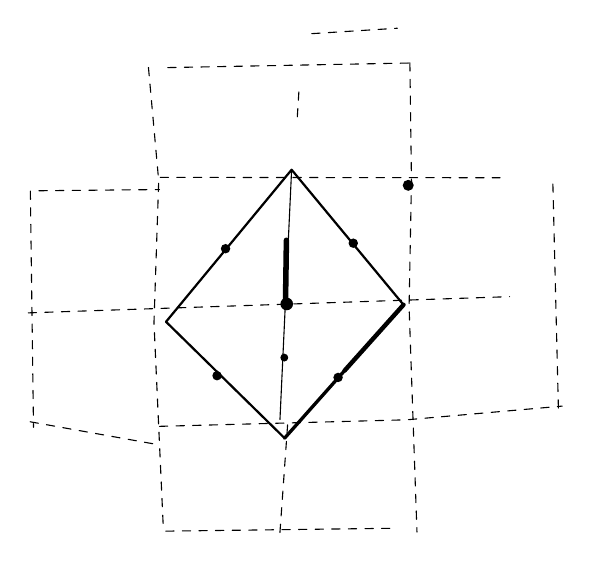
\begin{tikzpicture}[x=1mm,y=-1mm,line cap=round,line join=round,font=\small]
% dashed frame: the square (33-65 by 21.5-53) with its medians, a cell above and below (split by the vertical median), a cell left and right
\draw[dashed] (34.35,7.61) -- (65.53,7.02);
\draw[dashed] (52.64,3.3) -- (63.5,2.61);
\draw[dashed] (18,23.25) -- (33.3,23.1);
\draw[dashed] (33.39,21.55) -- (76.54,21.6);
\draw[dashed] (16.63,38.76) -- (77.76,36.7);
\draw[dashed] (16.87,52.59) -- (33.47,55.56);
\draw[dashed] (33.3,53.17) -- (64.71,52.34) -- (84.45,50.6);
\draw[dashed] (34.09,66.48) -- (63.35,66.11);
\draw[dashed] (31.9,7.6) -- (33.2,22) -- (32.6,40) -- (33.8,66.4);
\draw[dashed] (65.1,7) -- (65.3,22) -- (65,38) -- (66,66.6);
\draw[dashed] (16.9,23.3) -- (17.3,53.3);
\draw[dashed] (83.26,22.39) -- (83.97,51.22);
\draw[dashed] (51,10.7) -- (50.8,13.9);
\draw[dashed] (49.57,52.98) -- (48.58,66.9);
% the rhombus on the midpoints of the sides of the square
\coordinate (T) at (50.08,20.58);
\coordinate (R) at (64.29,37.73);
\coordinate (B) at (49.19,54.67);
\coordinate (L) at (34.13,39.89);
\draw[thick] (T) -- (R) -- (B) -- (L) -- cycle;
\draw[line width=1.6pt] (R) -- (56.8,46.1);
\draw[very thick] (56.8,46.1) -- (B);
% the vertical median inside the square, heavy from the centre halfway up
\draw[thin] (T) -- (48.6,52.3);
\draw[line width=2pt] (49.42,29.54) -- (49.3,37.6);
\fill (49.46,37.63) circle[radius=0.8];
\fill (41.69,30.61) circle[radius=0.6];
\fill (57.91,29.91) circle[radius=0.6];
\fill (40.61,46.74) circle[radius=0.6];
\fill (55.98,46.96) circle[radius=0.6];
\fill (49.15,44.44) circle[radius=0.5];
\fill (64.89,22.56) circle[radius=0.7];
\end{tikzpicture}
\end{document}
